\begin{figure}[t]
\centering
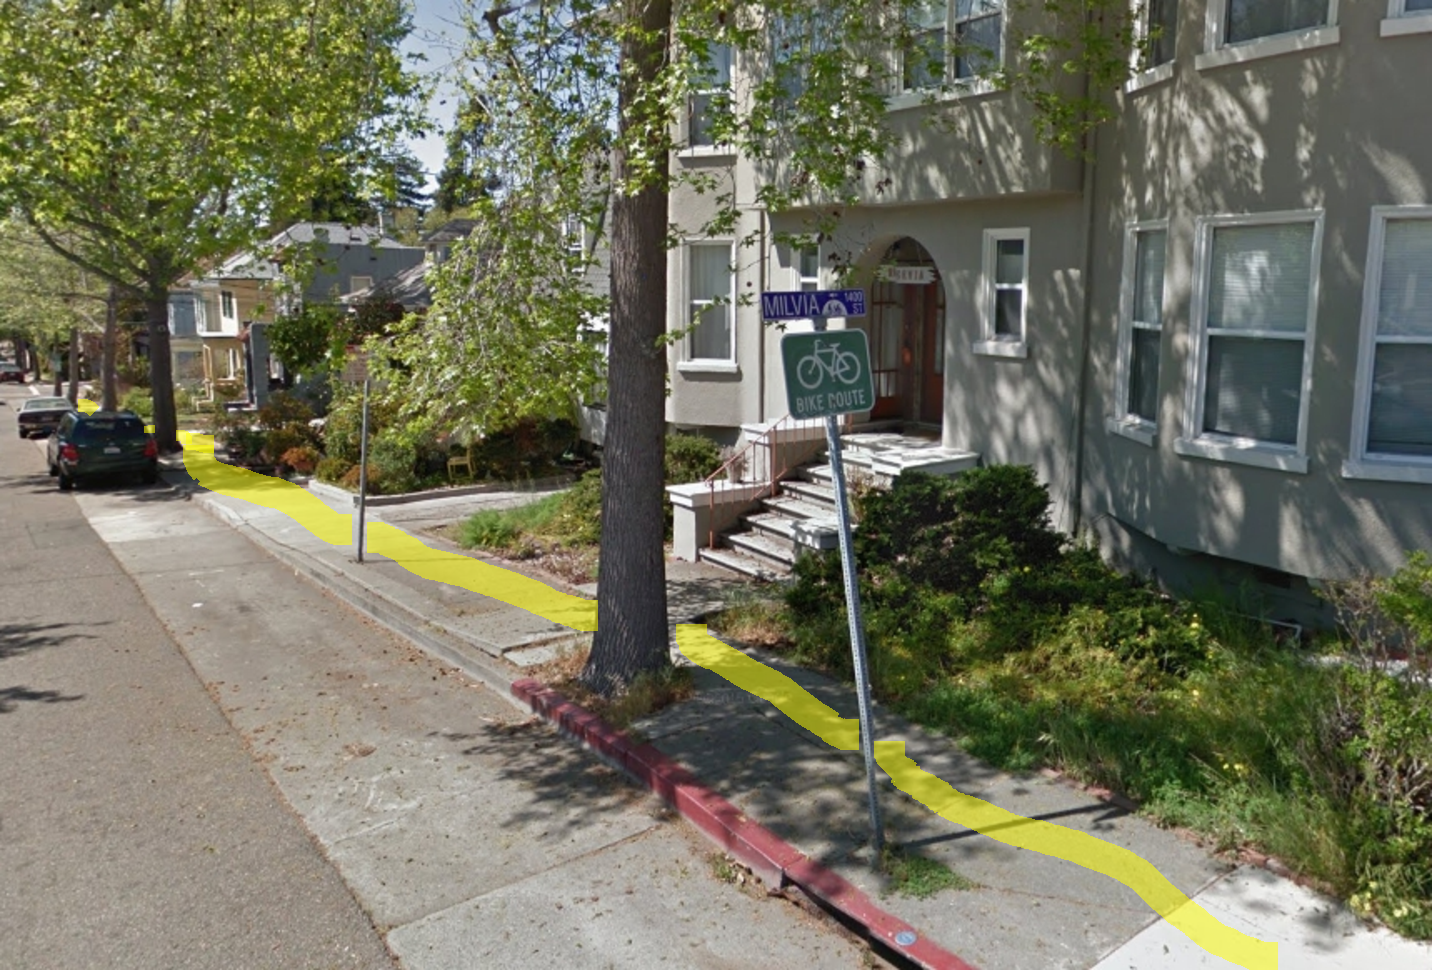
\includegraphics[width=\linewidth,,trim=0 0 0 0,clip]{paper/content/images/evaluation_path}
\caption{Segment of Evaluation Circuit}
\label{fig:evalpath}
\end{figure}

\section{CONCLUSION \& FUTURE WORKS}
\label{sec:conclusion}
This paper proposes a methodology for training DNNs to perform several distinct behavioral modalities simultaneously, through the insertion of modal information. This MultiNet approach is shown to exceed the performance of multiple individual networks trained separately, while using fewer parameters. These results are then verified with real world evaluation of the networks in sidewalk driving situations using 1/10th scale model cars. Future work could include work on adapting the approach to full size vehicles and making modal information available from higher-level networks trained to select behavioral modes, thereby granting the system a qualitatively higher level of autonomy.

\section*{ACKNOWLEDGMENTS}
The authors gratefully acknowledge NVIDIA for the donation of the NVIDIA TX1 Developer Kits, as well as Berkeley DeepDrive and it's sponsors for their support. We thank Sascha Hornauer and Eric Hou for their review, as well as Bhaskar Chowdhuri for assistance with figures.